%%%%%%%%%%%%%%%%%%%%%%%%%%%%%%%%%%%%%%%%%%%%%%%%%%%%%%%%%%%%%%%%%%%%%%%%%%%%%
%	e-Yantra, IIT-Bombay

%	Document Author: Abhishek Rathore, G. Harshawardhan
%	Date: 04-July,2016 

%%%%%%%%%%%%%%%%%%%%%%%%%%%%%%%%%%%%%%%%%%%%%%%%%%%%%%%%%%%%%%%%%%%%%%%%%%%%%

\documentclass[11pt,a4paper]{article}

\usepackage{graphicx}
\usepackage{listings}
\usepackage{url}
\usepackage{float}
\usepackage{subcaption}
\usepackage{hyperref}
\graphicspath{{../Images/}}
\title{Tutorial - Object Tracking (Based on ROI) and Re-recognizing the object if it escapes and comes back into the frame}
\author{e-Yantra Team}
\date{\today}

\begin{document}
	\maketitle
	\newpage
	\tableofcontents
	\newpage
	\section{Objective}
		This tutorial will teach you "How to track the object without errors based on ROI selection and How to re-recognize the object if it escapes and comes back inside the frame".
	\section{Prerequisites}
		User should have handy knowledge of the following for understanding this tutorial.
		\begin{itemize}
			\item Basics of Python.
			\item Basics of OpenCV.
			\item Basics of Image processing.
			\item CAMShift Algorithm (Refer to tutorial 2 to understand Camshift Algorithm).
		\end{itemize}
	\section{Hardware Requirement}
		\begin{itemize}
			\item A Computer with an internal or external webcam.
		\end{itemize}
	\section{Software Requirement}
		\begin{itemize}
			\item Python 2.7.11
			\item OpenCV 2.4.13 
			\item numpy 1.7.1
			\item \textbf{Note :} These are the versions we were working on while creating this tutorial.
		\end{itemize}
	\section{Theory and Description}
		 The base of algorithm used in this Tutorial is based on Camshift algorithm and this \href{http://vgl-ait.org/mdailey/uploads/publication_file/filename/106/Basit-CAMSHIFT.pdf}{research paper}. Details of Camshift algorithm can be found \href{https://github.com/eYSIP-2016/Object-Tracking-Camera/tree/master/Tutorials}{here}.
		 
		 The working of algorithm used for object tracking is described below.
		 \begin{itemize}
		 	\item First of all, it selects Region of Interest around Object, which you want to track using Mouse Callback function in Python. Mouse Callback function is shown in Figure 1.
			 	\begin{center}
			 		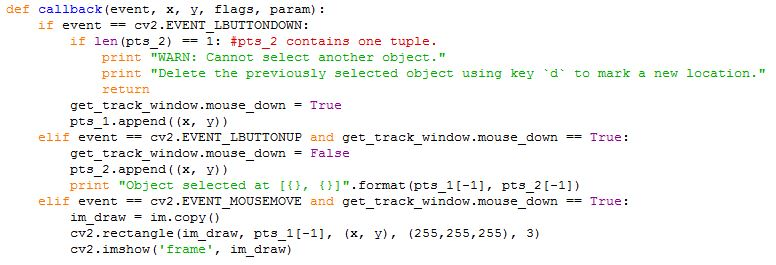
\includegraphics[scale=0.7]{Image4.JPG}
			 	\end{center}
			 	\begin{center}
			 		\textbf{Figure 1}
			 	\end{center}
		 	\item For selecting ROI press 'p', select region using mouse drag and then press 'p' to track that object. Figure 2 show initialization of ROI in video frame.
			 	\begin{center}
			 		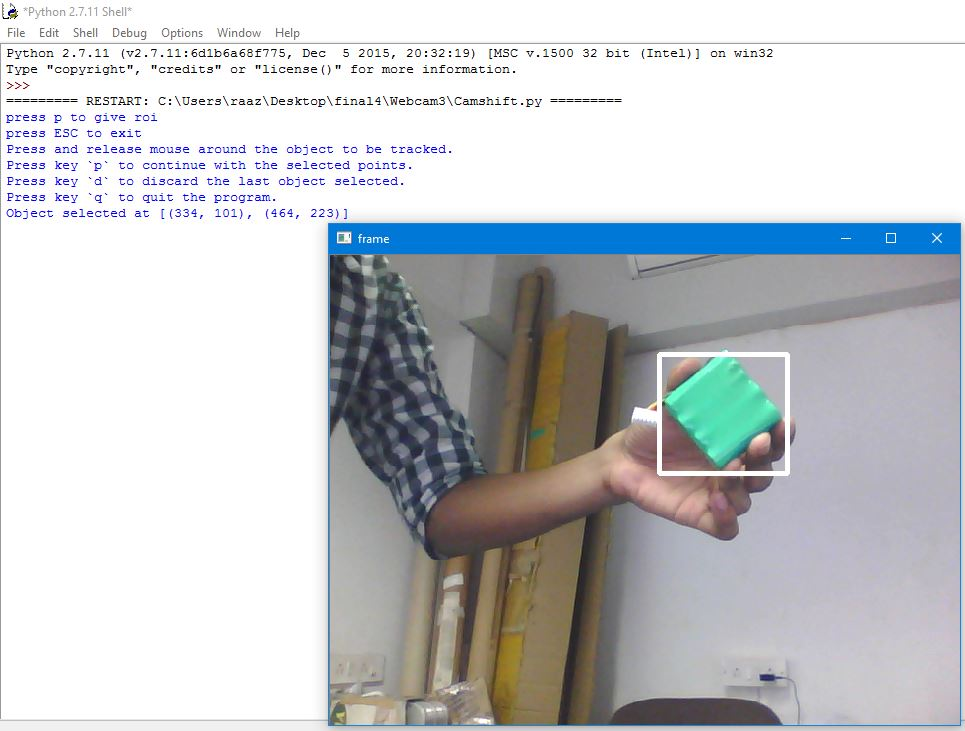
\includegraphics[scale=0.5]{giving_roi.JPG}
			 	\end{center}
			 	\begin{center}
			 		\textbf{Figure 2}
			 	\end{center}
		 	\item On pressing p it starts tracking the object by creating a bounding box around the object. Figure 3 shows tracking of object.
			 	\begin{center}
			 		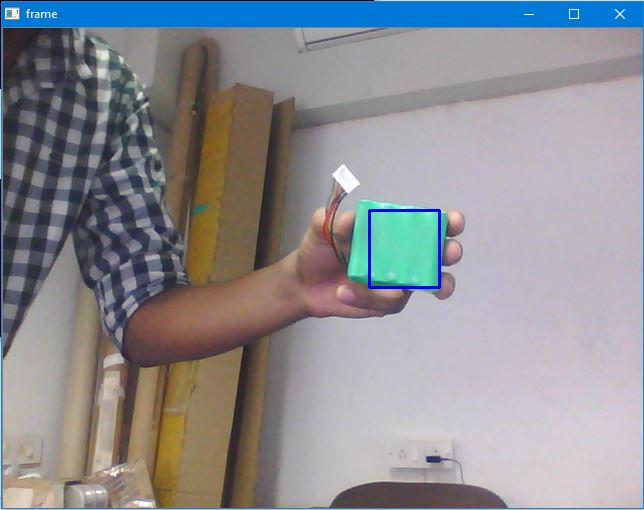
\includegraphics[scale=0.8]{tracking_object.JPG}
			 	\end{center}
			 	\begin{center}
			 		\textbf{Figure 3}
			 	\end{center}
			\item For tracking, it first calculate 2D histogram of selected Region Of Interest (HSV color space) only one time and stores it. Histogram means it is a graph which contains Hue values from 0 to 179 as y axis and Saturation values 0 to 255 as x axis and put number of pixels for each color. Here we uses normalized histogram in which all the values of number of pixels scaled to 0 to 1 using OpenCV functions. Code for calculation of histogram is shown in Figure 4 and calculated Normalized Histogram is shown in Figure 5.
				\begin{center}
					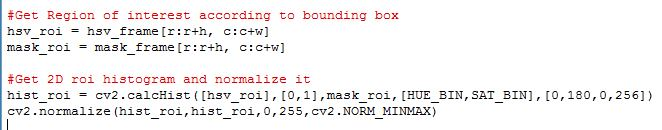
\includegraphics[scale=0.9]{roi_histogram_code.JPG}
				\end{center}
				\begin{center}
					\textbf{Figure 4}
				\end{center}
				\begin{center}
					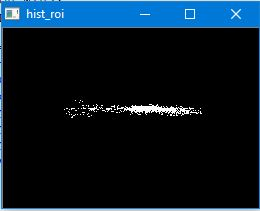
\includegraphics[scale=1]{histogram_roi.JPG}
				\end{center}
				\begin{center}
					\textbf{Figure 5}
				\end{center}
		 	\item Now it takes next frame and changes its color space from RGB to HSV and then eliminates the region of frame which was too far from the object in previous window using previous bounding box because sometimes Camshift Algorithm converges to other object of similar color of target object. Figure 6 shows code and Figure 7 shows Output image. We have considered that object movement will be real not very fast.
			 	\begin{center}
			 		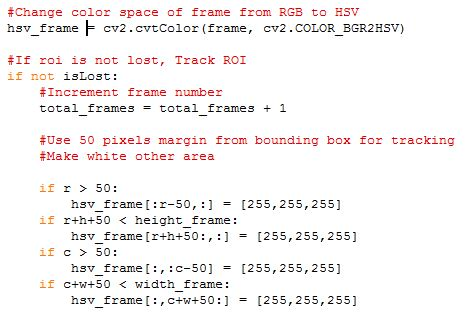
\includegraphics[scale=0.9]{frame_elimination_code.JPG}
			 	\end{center}
			 	\begin{center}
			 		\textbf{Figure 6}
			 	\end{center}
			 	\begin{center}
			 		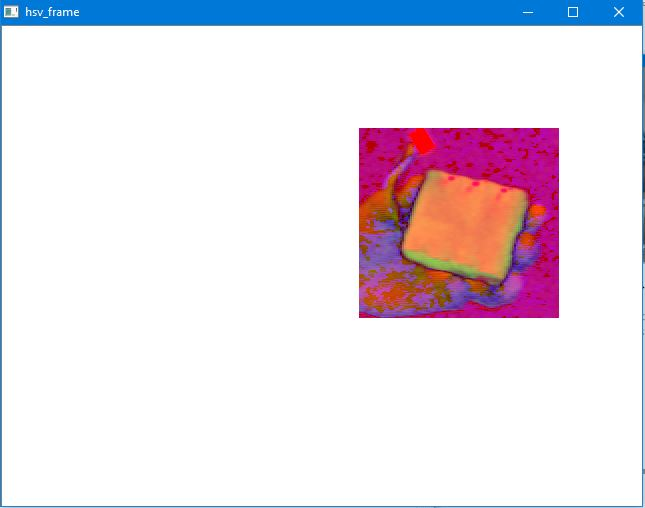
\includegraphics[scale=0.8]{eliminated_hsv_frame.JPG}
			 	\end{center}
			 	\begin{center}
			 		\textbf{Figure 7}
			 	\end{center}
			 \item Now it finds 2D Histogram of Figure 7, shown in Figure 9 using code shown it Figure 8.
				 \begin{center}
				 	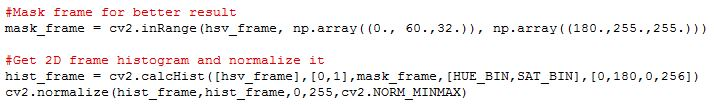
\includegraphics[scale=0.8]{frame_hist_code.JPG}
				 \end{center}
				 \begin{center}
				 	\textbf{Figure 8}
				 \end{center}
				 \begin{center}
				 	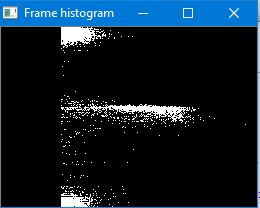
\includegraphics[scale=0.8]{frame_histogram.JPG}
				 \end{center}
				 \begin{center}
				 	\textbf{Figure 9}
				 \end{center}
			 \item Now it compares histogram of ROI and histogram of frame using Bhattacharya coefficient (OpenCV has inbuild function for it) and it gives histogram distance. Then calculates mean of the all the histogram distances. Then calculates standard deviation of mean. If current Histogram Distance follows the condition given in code (Figure 10), it means object is lost from window. Figure 10 shows code for this procedure.
				 \begin{center}
				 	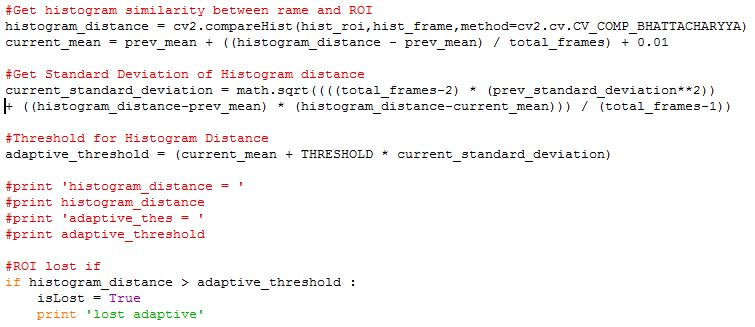
\includegraphics[scale=0.8]{code_histogram_comparison.JPG}
				 \end{center}
				 \begin{center}
				 	\textbf{Figure 10}
				 \end{center}
			 \item If condition is false back projection is calculated of HSV frame with respect to histogram of ROI. OpenCV provides function for back projection calculation. Then Camshift algorithm is applied to calculate new bounding box and minimum area ellipse. For more information about Camshift algorithm refer to Tutorial 2. Figure 11 shows code for it and Figure 12 shows back projection.
				 \begin{center}
				 	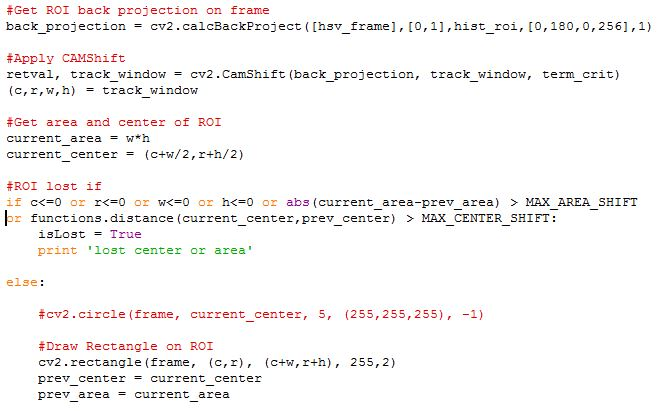
\includegraphics[scale=0.8]{camshift.JPG}
				 \end{center}
				 \begin{center}
				 	\textbf{Figure 10}
				 \end{center}
				 \begin{center}
				 	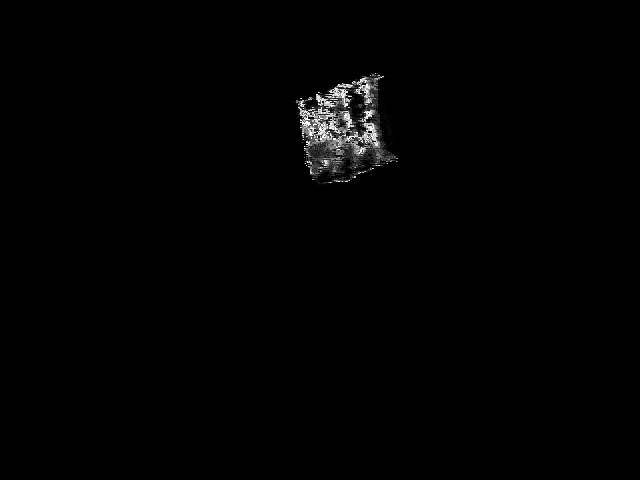
\includegraphics[scale=0.6]{back_projection.JPG}
				 \end{center}
				 \begin{center}
				 	\textbf{Figure 11: Back projection}
				 \end{center}
			 \item If object escapes from the frame then it show object is lost and continuously calculates back projection of frame, then binaries it and then uses erosion and dilation to remove errors and get big blobs of objects which has similar color as target object. Figure 12 show this back projection than we take contours in ]the back projection and get histogram of each contour in original frame. then compares these histograms with ROI histogram if one follows given condition given in Figure 13 code then it may be our object. Figure 12 shows code for redetection of object.
				 \begin{center}
				 	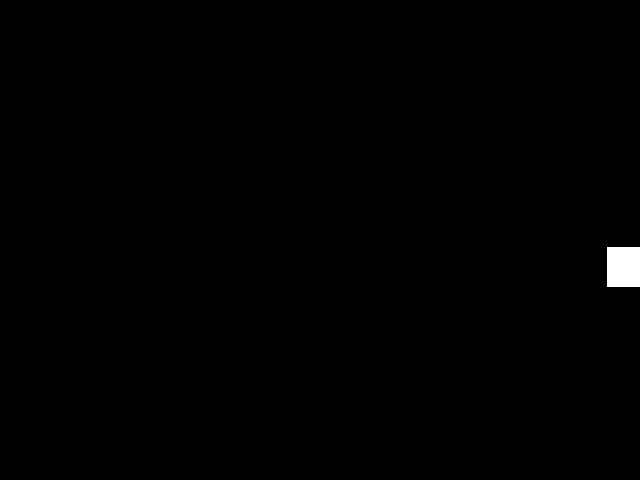
\includegraphics[scale=0.6]{special_back_projection.JPG}
				 \end{center}
				 \begin{center}
				 	\textbf{Figure 12: Eroded Dilated Binary Back projection}
				 \end{center}
				 \begin{center}
				 	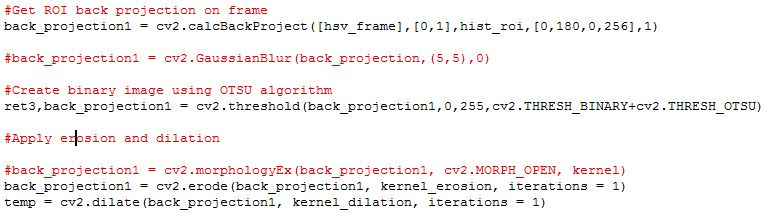
\includegraphics[scale=0.8]{redetection_back_projection.JPG}
				 \end{center}
				 \begin{center}
				 	\textbf{Figure 13(a): Redection part 1}
				 \end{center}
				 \begin{center}
				 	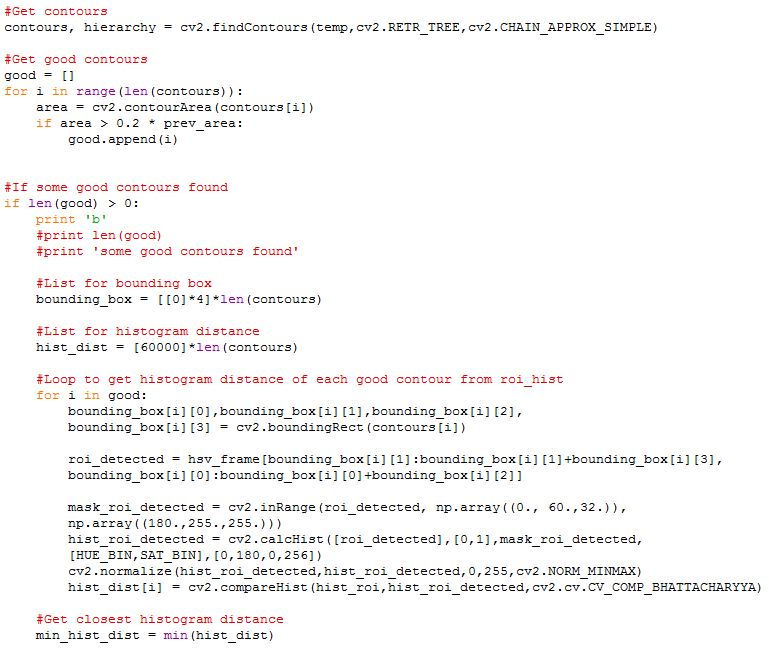
\includegraphics[scale=0.7]{redetection2.JPG}
				 \end{center}
				 \begin{center}
				 	\textbf{Figure 13(b): Redection part 2}
				 \end{center}
				 \begin{center}
				 	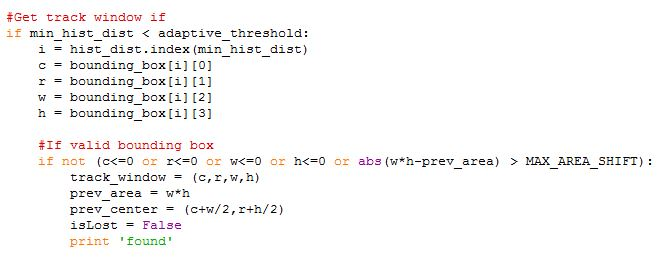
\includegraphics[scale=0.8]{redetection3.JPG}
				 \end{center}
				 \begin{center}
				 	\textbf{Figure 13(c): Redection part 3}
				 \end{center}
				 
			\item So this algorithm continuous above process iteratively and tracks the object frame by frame. 
		 \end{itemize}
	
	\section{Experiment}
	The Python code can be found \href{}{here}. To run code run run.py file and pause video by pressing 'p' and give roi and then track object by pressing 'p' again.
	\section{Exercise}
	Re-detection and tracking of an object  is shown below. In Figure 14 object is inside the frame. In Figure 15 object escapes from the frame. Then in Figure 16 It is again tracking the object.
	\begin{center}
		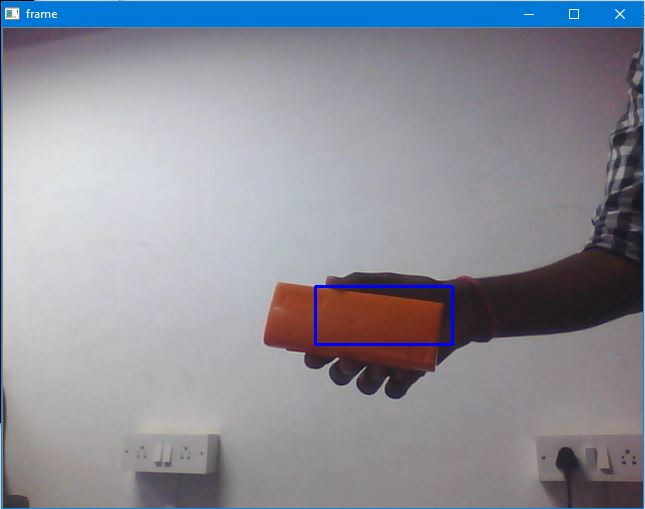
\includegraphics[scale=0.8]{Image1.jpg}
	\end{center}
	\begin{center}
		\textbf{Figure 14: Object is inside the frame}
	\end{center}
	\begin{center}
		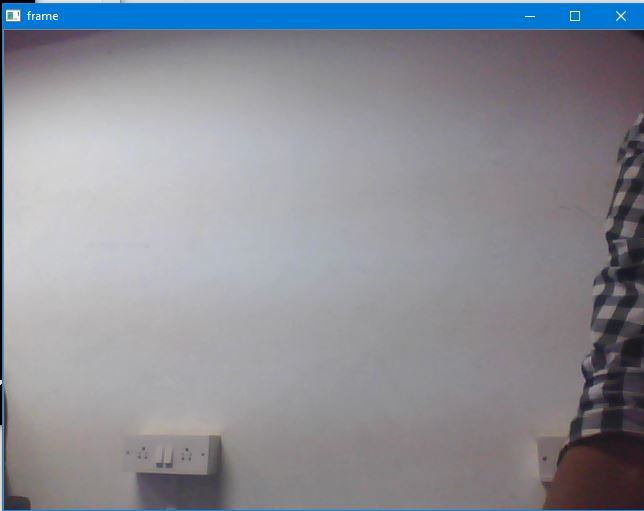
\includegraphics[scale=0.8]{Image2.JPG}
	\end{center}
	\begin{center}
		\textbf{Figure 15: Object lost in the frame}
	\end{center}
	\begin{center}
		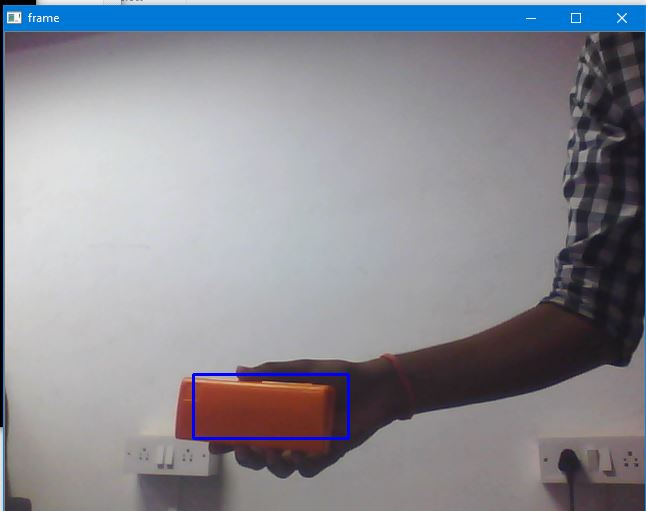
\includegraphics[scale=0.8]{Image3.JPG}
	\end{center}
	\begin{center}
		\textbf{Figure 16: Re-detection of object in the frame}
	\end{center}
	 In Figure 17 algorithm is not being confused because of the presence of similar colored object.
	 \begin{center}
	 	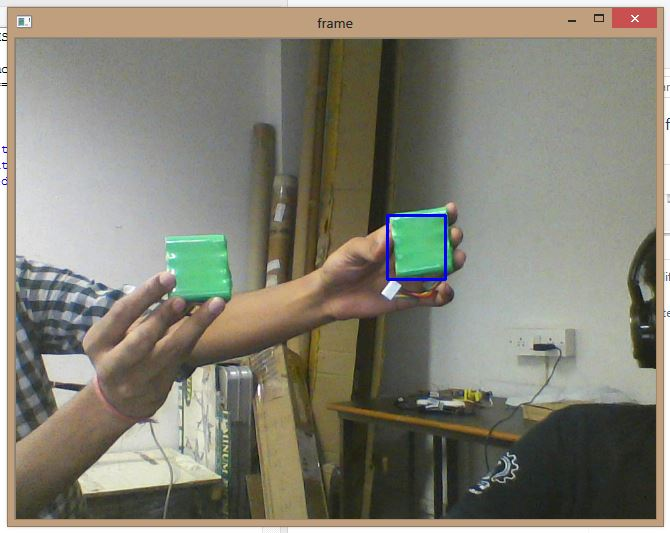
\includegraphics[scale=0.8]{test.JPG}
	 \end{center}
	 \begin{center}
	 	\textbf{Figure 17: Testing algorithm with similar colored object.}
	 \end{center}
	 \section{Limitations}
		 If similar colored object as color of your object is inside the frame then the algorithm will track the object but in presence of similar colored whole background it will say object is lost. If object is inside the frame after ROI selection, algorithm will track object in any scale and orientation. But if object escapes and comes back into the frame then it will be tracked if it will come to almost similar scale of object at the time of ROI selection.
	 \newpage
	\section{References}
	\begin{enumerate}
			\item \url{https://opencv-python-tutroals.readthedocs.io/en/latest/py_tutorials/py_tutorials.html}

\item \url{http://vgl-ait.org/mdailey/uploads/publication_file/filename/106/Basit-CAMSHIFT.pdf}
   \end{enumerate}
	
\end{document}



